\documentclass[12pt]{colt2019}

% The following packages will be automatically loaded:
% amsmath, amssymb, natbib, graphicx, url, algorithm2e

\title{The value of unlabeled data}
\usepackage{times}

\newcommand{\R}{\mathbb{R}}

\coltauthor{%
 \Name{Alexander Golovnev} \Email{alexgolovnev@gmail.com} \\
 \addr Harvard University, Cambridge, MA, USA
 \AND
 \Name{D\'avid P\'al} \Email{davidko.pal@gmail.com} \\
 \addr Yahoo Research, New York, NY, USA
 \AND
 \Name{Bal\'azs Sz\"or\'enyi} \Email{szorenyi.balazs@gmail.com} \\
 \addr Yahoo Research, New York, NY, USA
}

\begin{document}

\maketitle

\begin{abstract}
It has been shown that the amount of labeled examples to probably aproximately
learn a binary classifier decreases if the algorithm has access to the unlabeled
data. In particular, for the class of projections over $\{0,1\}^n$ there exists
a family of probability distributions such that learning any target concept with
access to unlabeled data requires only constant number of examples, but it
requires $\Omega(\log n)$ labeled examples in the worst case without the access
to unlabeled data. It remains an open problem to construct such distributions
and analyze the gap between the sample complexities for other important concept
classes such as half-spaces, axis parallel rectangles, disjunctions,
conjuctions, monotone disjunctions, monotone conjuctions.
\end{abstract}

\begin{keywords}
sample complexity, semi-supervised learning, probably approximately correct
learning
\end{keywords}

\section{Introduction}

The worst case sample complexity of probably approximately correct (PAC)
learning is very well understood~\citep{Hanneke-2016} and it is known to be
$\Theta \left(\frac{d + \log(1/\delta)}{\epsilon}\right)$ where $d$ is the
Vapnik-Chervonenkis dimension, $\epsilon$ is the accuracy parameter and $\delta$
is the confidence parameter. Similarly, the sample complexity of learning under
a fixed distribution $P$ is reasonably well understood~\citep{Benedek-Itai-1991}
and it is between $\Omega(\log(M_{2\epsilon}) + \log(1-\delta))$ and $O
\left(\frac{\log N_{\epsilon/2} + \log(1/\delta)}{\epsilon} \right)$, where
$M_{2\epsilon}$ is the size of an $2\epsilon$-packing of the concept class with
respect to the disagreement metric $d_P(f,g) = \Pr_{x \sim P}[f(x) \neq g(x)]$
and $N_{\epsilon/2}$ is the size of an $\frac{\epsilon}{2}$-cover of the concept
class with respect to same metric.

The sample complexity of learning under a fixed distribution depends on the
distribution, while the worst case complexity of PAC learning does not. See
Figure~\ref{figure:sample-complexity}. For some distributions the sample
complexity of fixed distribution learning is much lower than the (worst-case)
PAC sample complexity.

\begin{figure}
\centering
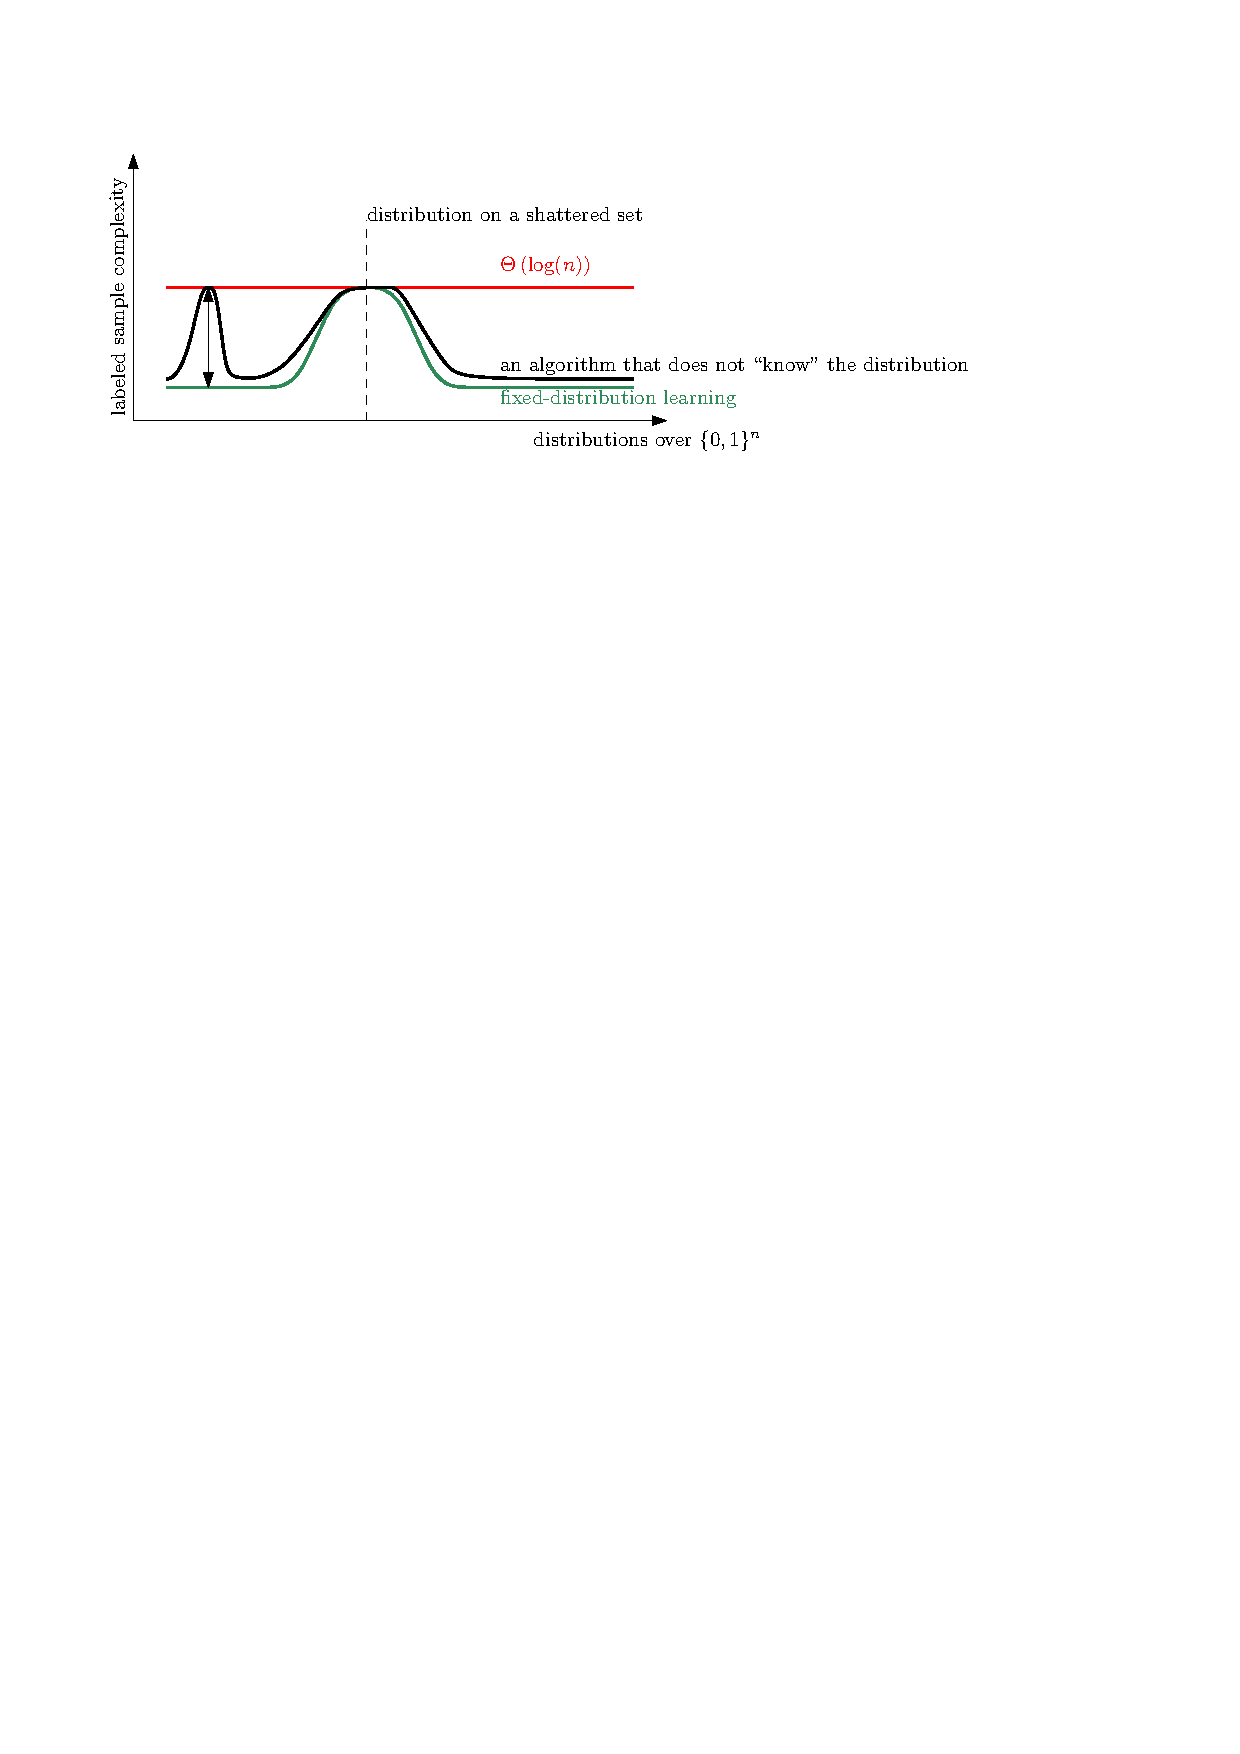
\includegraphics[scale=1.0]{figure}
\caption{The graph shows sample complexity bounds of learning a class of
projections over the domain $\{0,1\}^n$ under various unlabeled distributions.
We assume that $\epsilon$ and $\delta$ are constant, say, $\epsilon = \delta =
\frac{1}{100}$. The graph shows three lines. The red horizontal line is PAC
sample complexity bound for the class of projections, which is $\Theta(\log n)$.
The green line is the Benedek-Itai bound. The green line touches the red line
for certain distributions, but is lower for other distributions. In particular,
for certain distributions the green line is $O(1)$. The dashed line corresponds
to a particular distribution on a shattered set. This is where the green line
and red line touch. Furthermore, here the upper bound coincides with the lower
bound for that particular distribution. The black line is the sample complexity
of an arbitrary \emph{distribution-independent} algorithm. For example, the
reader can think of the ERM or Hanneke's algorithm.
\cite{Golovnev-Pal-Szorenyi-2019} proved that there exist a distribution where
the black line is $\Omega(\log n)$ times higher than the green line. This
separation is indicated by the double arrow.}
\label{figure:sample-complexity}
\end{figure}

Existing algorithms for learning under a fixed distribution depend in a
non-trivial way on the distribution in question. On the other hand PAC learning
algorithms do \emph{not} depend on it. It is thus a natural question to ask
whether or not the access to unlabeled data is necessary in order to match the
lower sample complexity attained in the fixed distribution learning setting.

This question was studied by \cite{Darnstadt-Simon-Szorenyi-2013} and
\cite{Golovnev-Pal-Szorenyi-2019}. They have shown that having access to
unlabeled data is beneficial for the class of projections over $\{0,1\}^n$. More
specifically, there exists a family of distributions such that any target
projection is fixed distribution learnable with constant number of samples,
however any learner that does not have access to the unlabeled data needs
$\Omega(\log n)$ examples in the worst case.

It remains an open problem to analyze other concept classes of interest.
Specifically, it is unknown what is the gap, if any, for the classes of
half-spaces and axis parallel rectangles over $\R^n$, disjunctions, conjuctions,
monotone disjunctions and monotone conjuctions over $\{0,1\}^n$. While sample
complexity depends on the accuracy parameter $\epsilon$ and confidence parameter
$\delta$, we are primarily interested in the dependency on the dimension $n$.

We conjecture that there is gap at least $\Omega(\log n)$, but it is possible
that the gap is as high as $\Omega(n^\alpha)$ for some $\alpha \in (0,1]$. In
order to show the existence of a gap, one must construct a family of
distributions such that fixed distribution learning has low sample complexity
but worst-case sample complexity without knowledge of the distribution is
higher.

We remark that the Vapnik-Chervonenkis dimension of projections is only
$\Theta(\log n)$, while the Vapnik-Chervonenkis dimension of the above-mentioned
concept classes is $\Theta(n)$.  This suggests that a different construction is
needed. We offer \$100 USD for the first solution of this problem for at least
one of these concept classes.

\bibliography{biblio}

\end{document}
